\section{EMPIRICAL EVALUATION}
\label{sec:results}
In this section, we evaluate our proposed system by analyzing the predictive performance and communication complexity  using a real-world event streams provided by the datAcron project in the context of maritime monitoring. The used event streams describe critical points (i.e., synopses) of moving vessels trajectories, which are derived from raw AIS messages as described in \cite{synopses1}. In particular, for our evaluation experiments we used a data set of synopses contains $4,684,444$ critical points of $5055$ vessels sailing in the Atlantic Ocean during the period from 1 October 2015 to 31 March 2016. We used it to generate a simulated stream of event tuples  i.e., \textit{(id,timestamp, longitude, latitude, annotation, speed, heading)}, which are processed by the system to attach an extra attribute \textit{type} that represents the event value,  where $type$ $\in \Sigma$,  and $ \Sigma= \Sigma_1=$$\{$\textit{VerySlow ,Slow, Moving, Sailing, Stopping} $\}$ , which is based on ranging the speed values. Or $\Sigma=\Sigma_2=$ $\{$  \textit{stopStart,stopEnd, changeInSpeedStart, changeInSpeedEnd, slowMotionStart, slowMotionEnd, gapStart, gapEnd,   changeInHeading} $\}$, which is derived based on the values of the $annotation$ attribute that encodes the extracted trajectory movement events \cite{synopses1}. In our experiments, we monitor a pattern $\mathcal{P}_1=Sailing$ with $\Sigma_1$ that detects when the vessel under way (sailing). Likewise, we test a second pattern  $\mathcal{P}_2=$\textit{changeInHeading; gapStart; gapEnd; changeInHeading} with $\Sigma_2$.


\subsubsection*{Experimental setup} We ran our experiments on single-node standalone Flink cluster deployed on an Ubuntu Server 17.04 with Intel(R) Core(TM) i7-7700 CPU @ 3.60GHz X 8 processors and 32GB RAM. We used Apache Flink v1.3.2 and Apache Kafka v0.10.2.1 for our tests.


\subsubsection*{Evaluation criteria} Our goal is to evaluate our distributed pattern prediction system, which enables the synchronization of prediction models(i.e., PMC models) on the distributed predictor nodes. Our proposed system can operate in three different modes of synchronization protocols/schemes: \begin{enumerate*}[label=(\roman*)] 
	\item static scheme based on synchronizing the prediction models periodically every $b$ of input events, 
\item continuous synchronization for each incoming event (hypothetical), 
\item dynamic synchronization protocol based on making the predictors communicate their local prediction models periodically only when the divergence of the local models form a reference model exceeds a variance threshold $\Delta$ (recommended).
 	   
\end{enumerate*}
We compare our proposed system against the isolated prediction approach, we compare the predictive performance in terms of :
\begin{enumerate*}[label=(\roman*)]
	
\item  $\mathit{precision = \frac{\#\ of\ correct\ predictions}{\#\ of\ total\ predictions}}$ is the percent of the produced predictions are correct (i.e., a full match occurred within the prediction interval).   

\item $\mathit{recall}$ is the fraction of the full matches of the pattern are successfully predicted by the system at least once. 

\end{enumerate*} 
\par Moreover, we study the communication cost by measuring the $\mathit{cumulative\ communication}$ that captures the number of messages are required to perform the distributed online learning modes to synchronize the prediction models. In next, we present the experimental results for the patterns  $\mathcal{P}_1=Sailing$ with an order of $m=2$, and   $\mathcal{P}_2=$\textit{changeInHeading; gapStart; gapEnd; changeInHeading} with first order $m=1$. As well as all experiments are performed with batch size equals 100  ($b=100$), a variance threshold of 2 ($\Delta=2$), and $80\%$ as PMC prediction threshold ($\theta_{fc}=80\%$).

\begin{figure}[h]
	
	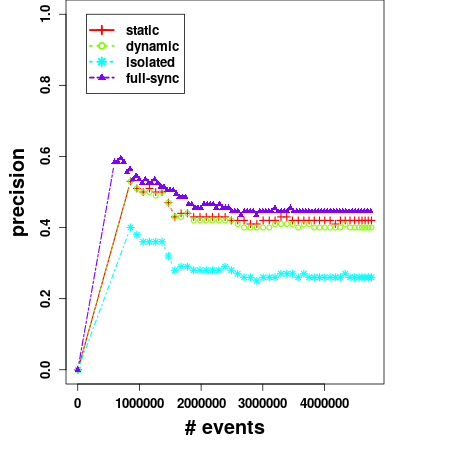
\includegraphics[width=.5\textwidth]{figures/precision.png}
	
	\caption{Precision scores with respect to the number of input events over time for $\mathcal{P}_1$.}
	\label{fig:precsions}
\end{figure}

\subsubsection*{Experimental results} Figure ~\ref{fig:precsions} depicts the average precision scores of predictions models (one prediction model per vessel) of all approaches for the first pattern $\mathcal{P}_1=Sailing$, namely, isolated without synchronization, continuous (full-sync), static, and our recommended approach based on the dynamic synchronization scheme. It can be clearly seen that all methods of distributed learning outperform the isolated prediction models. The most complex method, continuous synchronization, has the higher precision rates, while the static and dynamic synchronization schemes have a close precision scores.

In addition, we have found that in order to have an improvement in terms of precision for the second pattern ($\mathcal{P}_2$), a slight modification is needed that to only enable the synchronization of the prediction models associated with vessels that belong to the same type. Currently, this change is technically performed by an extra filter step that passes only one type of vessels at time, while multiple runs of the system are required for all vessel types. Fore example, Figure ~\ref{fig:precsions_p2} shows the precision scores for vessels of type \textit{PLEASURE CRAFT}. An interesting observation is that the dynamic synchronization approach has the higher precision scores.  

 \begin{figure}[h]
 	
 	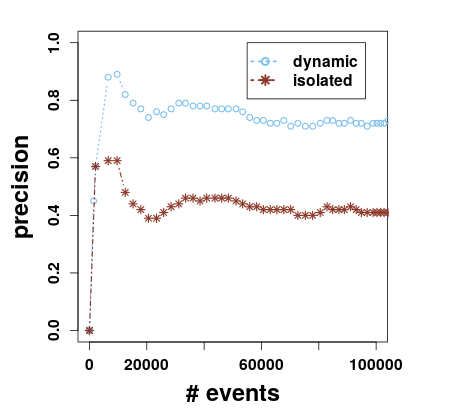
\includegraphics[width=.5\textwidth]{figures/precision_p2.png}
 	
 	\caption{Precision scores of $\mathcal{P}_2$  for \textit{PLEASURE CRAFT} vessels.}
 	\label{fig:precsions_p2}
 \end{figure}
 
 
\par On the other hand, Figure ~\ref{fig:comm} provides the amount of the accumulated communication that is required by the three modes of the distributed online learning, while, the isolated approach does not require any communication between the predictors. These results are shown  $\mathcal{P}_1$, while we have omitted the measurements of  $\mathcal{P}_2$ since it has shown a similar behavior.  As expected, a larger amount of communication is required for the continuous synchronization comparing to the static and dynamic approaches, and it can bee seen that we can reduce the communication overhead by applying the dynamic synchronization protocol (a reduction by a factor of 100) comparing to the static synchronization scheme, even with a small variance threshold $\Delta=2$. Furthermore,  the dynamic  protocol is still preserving a close predictive performance to the static one (see Figure ~\ref{fig:precsions}).    


\begin{center}
	
	\begin{figure}[h]
		
		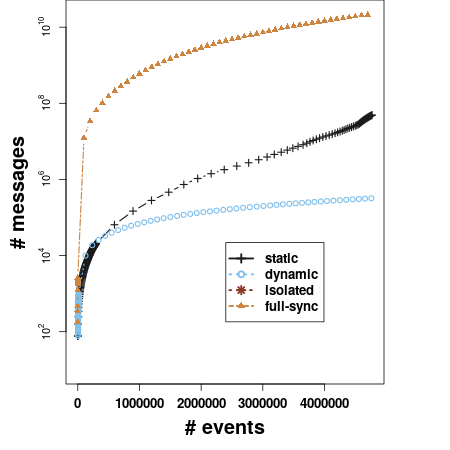
\includegraphics[width=.5\textwidth]{figures/communication.png}
		
		\caption{Commutative communication with respect to the number of input events over time for $\mathcal{P}_1$.}
		\label{fig:comm}
	\end{figure}
\end{center}

\par In Table ~\ref{tab:recall}, we present the mean of the recall scores for the both patterns in the all approaches It can be seen that the different approaches have a close recall scores, while the most frequent pattern ($\mathcal{P}_1$) has a lower recall than $\mathcal{P}_2$.

\begin{table}[h]
	\caption{Average recall for  $\mathcal{P}_1$ and $\mathcal{P}_2$.}
	\label{tab:recall}
	\begin{tabular}{lcc}
		\toprule
		Approach &Mean recall for $\mathcal{P}_1$ &Mean recall for $\mathcal{P}_2$\\
		\midrule
		isolated & 0.1707  &0.947 \\
		static & 0.1754  &  0.960 \\
		dynamic & 0.174  & 0.0.964 \\
		full-sync & 0.1817  & 0.972 \\
		\bottomrule
	\end{tabular}
\end{table}


 
